\section{Implementing CustomGraphSearch}
 %\setcounter{page}{2}
 %\addtocounter{section}{1}
 \thispagestyle{empty}
\subsection{Aim}

This second lab session explores the concept of graph search algorithms. The
agent is still a Vacuum cleaner evolving in a simple grid.
Each square of that grid is either clean filled with dirt, or a wall.
The vacuum cleaner uses search algorithm to locate the dirt squares.
The purpose of this lab is to write our own implementation of
\textit{Breadth First Search} and \textit{Depth First Search} algorithms which
inherit from a \textit{CustomGraphSearch} class.

Using the Java GUI included in the project files, it is possible to compare the
efficiency of differents search algorithms : BFS, DFS, IDS, A*.

%\begin{itemize}
%  \item Turning 90° in the given direction (\textit{uMovement equal to 0})
%  \item Moving forward, down to the next grid line (\textit{uMovement equal to 1})
%  \item Turning again in the same direction (\textit{uMovement equal to 0 again})
%\end{itemize}

\subsection{Implementation}

Given that the course book and the slides provide us with pseudo code of the
algorithms, it is easier to realize the implementation.



\begin{figure}[h]
    \centering
    \begin{tabular}{cc}
      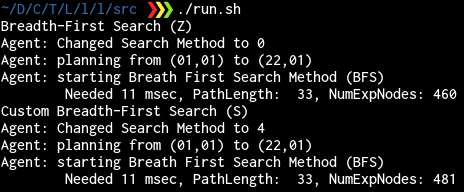
\includegraphics[width=.44\linewidth,scale=1]{./images/lab2_bfs.png} & 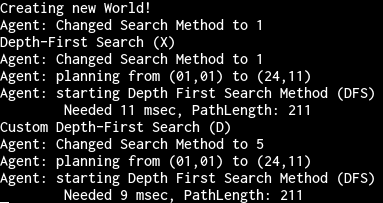
\includegraphics[width=.36\linewidth, scale=1.5]{./images/lab2_dfs.png} \\
      \hspace{0.5cm} (a) & \hspace{0.5cm} (b)
    \end{tabular}
    \caption{Comparison between builtin and custom implementation (a) BFS - (b) DFS \label{fig:BFS and DFS}}
\end{figure}

%\begin{figure}[h]
%    \centering
    %  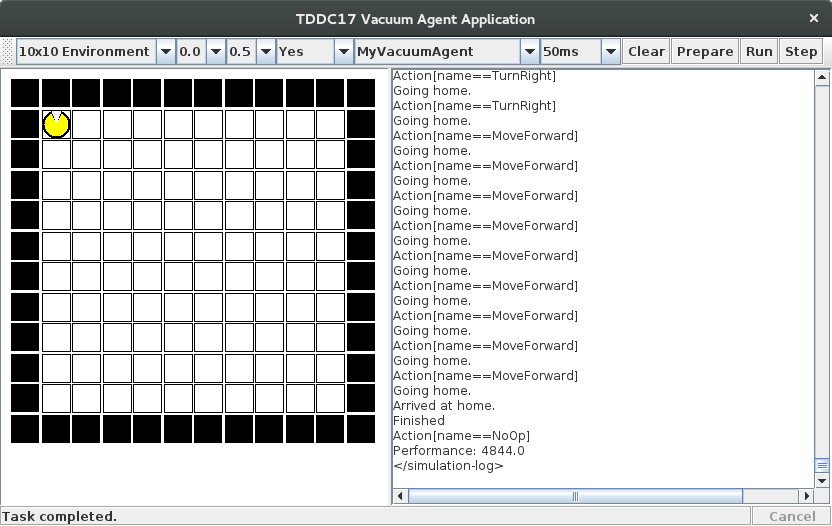
\includegraphics[width=0.83\linewidth]{./images/lab_1.png}
  %  \caption{Screenshot\label{Vacuum cleaner}}
%\end{figure}

\newpage
\thispagestyle{empty}
\section{Theory}

\paragraph{Question 1}
\paragraph{Question 2}
\paragraph{Question 3}
\paragraph{Question 4}
\paragraph{Question 5}
\paragraph{Question 6}
\paragraph{Question 7}
